\chapter{Numerical Simulations}%
\label{chapter:five}
In order to test the implemented \texttt{UMAT} subroutines  for the viscoelastic material model, numerical simulations were carried out in ABAQUS. To this end, finite element models with both a single element and multiple elements were considered. Here, material parameters identified in \cref{tab:opt_param_sets} for the dual cross-link self-healing hydrogel material were used.

\section{Single-Element Simulations}
Using a model with a single finite element, it is possible to test the developed \texttt{UMAT} and check for any implementation errors. For this, a uniaxial tension test mimicing the experimental data in \cref{fig:uniaxial_experiments} was simulated using one C3D8H\footnote[1]{8-noded 3D continuum element with hybrid formulation in ABAQUS} element of size 10mm x 10mm x 10mm.

Firstly, the element was fixed \((u_{x}, u_{y}, u_{z} = 0)\) on one end \((x=0)\) and a ramp displacement of 10mm was applied in the x-direction with a constant displacement rate on the other end \((x=10)\). The constant displacement rate 
\begin{equation}
    \dot{u}_{x} = \mathrm{L}_{0} \dot{\lambda_{x}}
    \label{eq:displacement_rate}
\end{equation}
was derived from the stretch rate given the fact that
\begin{equation}
     \lambda_{x} = 1 + \dfrac{{u_{x}|}_{x=10}}{\mathrm{L}_{0}}
\end{equation}  where \(L_{0} = 10\). 
In order to compare the results with the experimental data and the twin implementation in MATLAB, the simulations were carried out for stretch rates ranging from \(0.1s^{-1}\) to \(0.003s^{-1}\). Furthermore, the implemented viscoelastic material models with, both, two \((k=2)\) and three \((k=3)\) relaxation mechanisms were used. It was found that, the response of the material model was affected by the stretch rates as seen in \cref{fig:abaqus_comparison}, which was as expected. However, for both the models (2EL and 3EL), the material response was not in agreement with the experimental data. The reason for this contradiction could either be the fact that, ABAQUS implements logarithmic strains for problems with large deformation, or, that the finite element formulation used in ABAQUS differs from the purely analytical approach that was used to calculate the material response in MATLAB during the parameter identification procedure. It is also possible that experimental data from multiple loading cases is required for identifying the optimal set of parameters\cite{Kleuter2007Jul}. Nevertheless, this needs further investigation. One possible way to avoid this deviation would be to use ABAQUS to calculate the material response instead of MATLAB for the cost function in \cref{eq:unconstrained_optimization}. This, however, is also not dealt with in this work.

\begin{figure}[htpb]
    \centering
    \subfloat[]{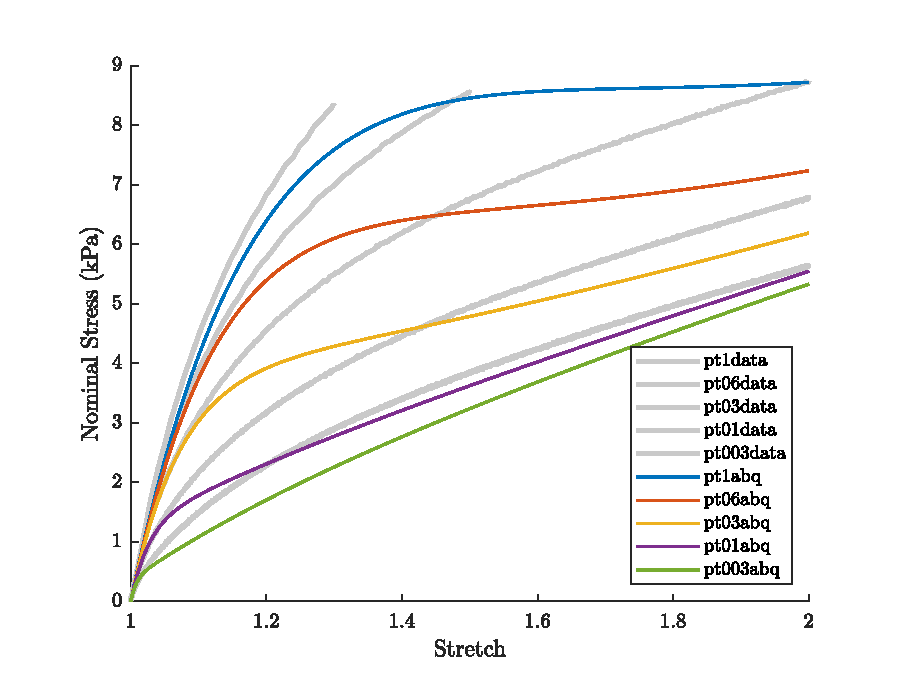
\includegraphics[width = 0.85\textwidth]{2EL_Abaqus_NR.eps}} \label{fig:abaqus_comparison_2EL}
    \subfloat[]{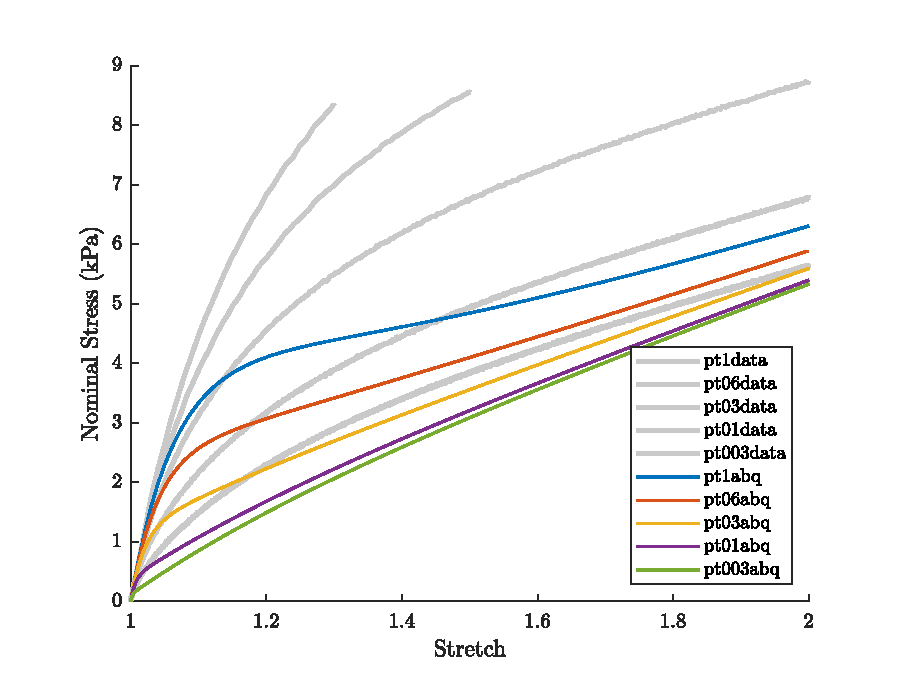
\includegraphics[width = 0.85\textwidth]{3EL_Abaqus_NR.eps}} \label{fig:abaqus_comparison_3EL}\\
    \caption[Uniaxial tension test simulation]{Uniaxial tension test simulation in ABAQUS using viscoelastic material model (a) with two relaxation mechanisms \((k=2)\) and (b) with three relaxation mechanisms \((k=3)\) and respective material parameters \(\bm{x}_{p}\) for \(2\mathrm{EL}_{\mathrm{NR}}\), \(3\mathrm{EL}_{\mathrm{NR}}\) taken from \cref{tab:opt_param_sets}}
    \label{fig:abaqus_comparison}
\end{figure}

Next, the single element model was subjected to uniaxial loading followed by unloading. In this case, the element was fixed \((u_{x}, u_{y}, u_{z} = 0)\) on one end \((x=0)\).  On the other end \((x=10)\) a ramp displacement of 10mm followed by a negative ramp displacement of 10mm was applied in the x-direction with a constant displacement rate  given by \cref{eq:displacement_rate}. Here, again the simulations were carried out for stretch rates varying from \(0.1s^{-1}\) to \(0.003s^{-1}\). For this simulation, only the viscoelastic material model with two relaxation mechanisms \((k=2)\) was used. The material response for the simulations is given in \cref{fig:loading_unloading_abaqus}. Here, it can be seen that the material response is generally affected by the stretch rates. Furthermore, during unloading, the nominal stress \(\mathrm{P}_{11} = 0\) for stretch \(\prstretche{}{1} > 1\). This effect is desired and is also in agreement with the  material model developed by \citeauthor{Long2014Oct} \cite{Long2014Oct} for the hydrogel material at hand.

\begin{figure}[htbp]
    \centering
    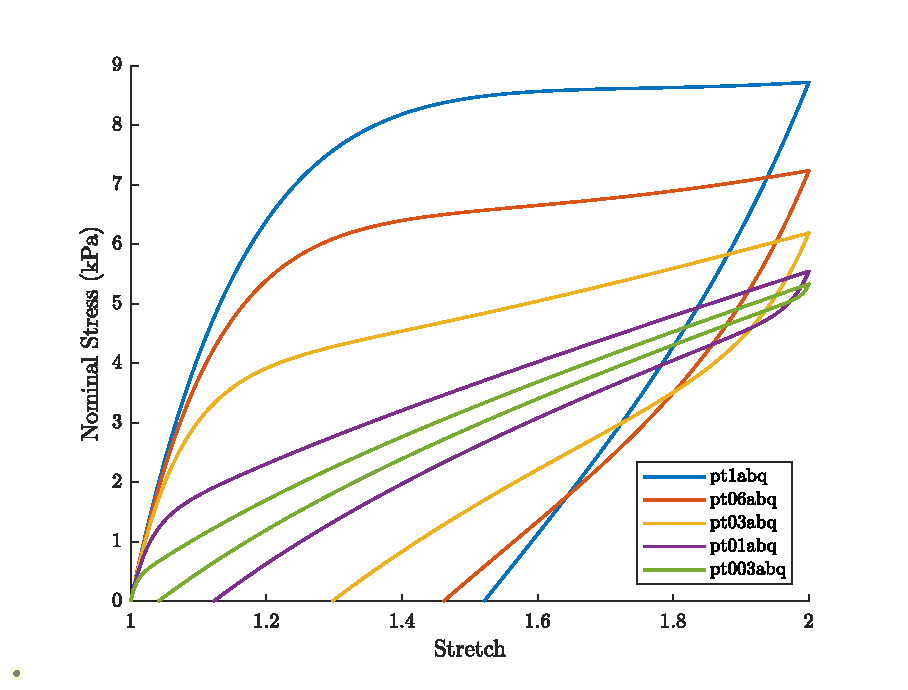
\includegraphics[width=0.95\textwidth]{2EL_loading_unloading_Abaqus.eps}
    \caption[Uniaxial loading and unloading simulation]{Uniaxial loading-unloading simulation in ABAQUS for viscoelastic material model with two relaxation mechanisms \((k=2)\) using material parameters \(\bm{x}_{p}\) for \(2\mathrm{EL}_{\mathrm{NR}}\) (\cref{tab:opt_param_sets}) }%
    \label{fig:loading_unloading_abaqus}
\end{figure}

Finally, the single element model was subjected to uniaxial loading and relaxation. Here, again the element was fixed \((u_{x}, u_{y}, u_{z} = 0)\) on one end \((x=0)\). On the other end \((x=10)\), a ramp displacement of 10mm was applied in the x-direction with a constant displacement rate given by \cref{eq:displacement_rate}. At the end of this step, the displacement was held constant at 10mm and the material was allowed to relax. For this simulation too, only the implemented viscoelastic material model with two relaxation mechanisms \((k=2)\) was used. The material response for the simulations is given in \cref{fig:loading_relaxation_abaqus}. Here during the relaxation phase, it can be seen that after certain time, the stress \(\sigmatot\), and hence, \(\mathbf{P}\) within the element reduces to the equillibrium stress \(\sigmaeq\), and hence \(\mathbf{P}_{\mathrm{EQ}}\), which is expected behaviour for a viscoelastic material model. 

\begin{figure}[htbp]
    \centering
    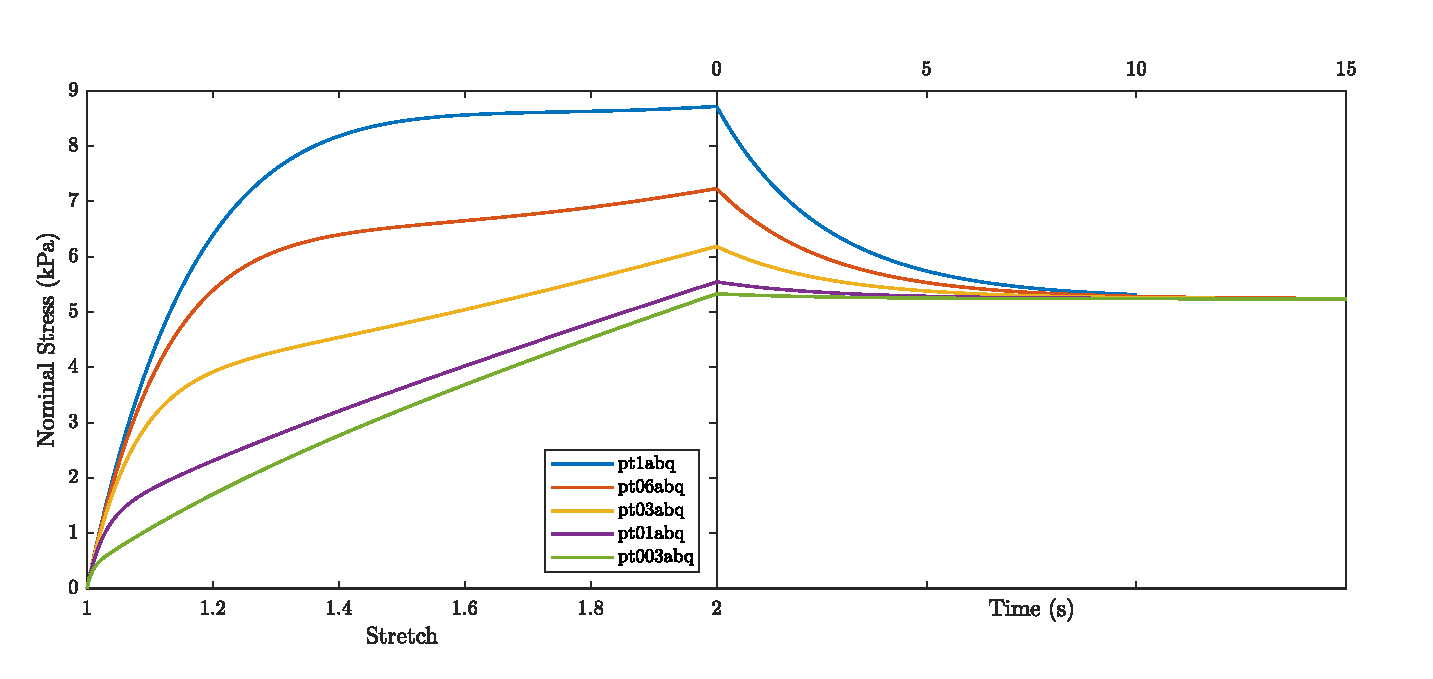
\includegraphics[width=1\textwidth]{2EL_loading_relaxation_Abaqus.eps}
    \caption[Uniaxial loading and relaxation simulation]{Uniaxial loading-relaxation simulation for viscoelastic material model in ABAQUS  with two relaxation mechanisms \((k=2)\) using material parameters \(\bm{x}_{p}\) for \(2\mathrm{EL}_{\mathrm{NR}}\) (\cref{tab:opt_param_sets})}%
    \label{fig:loading_relaxation_abaqus}
\end{figure}

\section{Multi-Element Simulations}
Now that the implemented viscoelastic material models demonstrated the expected behaviour in finite element models involving a single element, they were further tested with finite element models involving multiple elements. To this end, a column twisting simulation with a pressure-follower load as described in \cref{fig:twister} was employed\cite{Bonet2015Jan}. The column was 6mm tall and had a cross section of 1mm~x~1mm. An additional section of 3mm~x~1mm~x~1mm on the top was used to apply the pressure-follower load. The response of the model was then observed at the point \(A \equiv (1.0, 0.0, 6.5)\). The geometry was discretized with a mesh size of 0.25mm or 0.1mm resulting in 576 and 9000 elements respectively. Furthermore, both C3D8H and C3D20H\footnote[1]{20-noded 3D continuum element with hybrid formulation in ABAQUS} element formulations were employed.

\begin{figure}[htbp]
    \centering
    \includegraphics[width=0.9\textwidth]{twister_} 
    \caption[Column twisting simulation]{Column twisting simulation model definition using pressure-follower load (left) and exemplary deformed shape (right)}%
    \label{fig:twister}
\end{figure}

The response of the column twisting simulations is as shown in \cref{fig:column_twisting}. In the case of \emph{slow} simulations, the pressure was ramped at a rate of 2.5~kPa/s and 1.5~kPa/s for simulations with C3D8H and C3D20H elements respectively. For all other simulations, the pressure was ramped at a rate of 1~MPa/s. It is evident from the results that the invariants of the Cauchy stress tensor \(I_{\sigmatot}, II_{\sigmatot}, III_{\sigmatot} \text{ and } II_{\mathrm{dev}(\sigmatot)}\) are affected by the rate of deformation or  the rate of pressure application. The stress invariants for simulations with slower pressure application rate were always lower. This is because at slower rates of deformation or pressure application, the contribution of the non-equillibrium stress \(\sigmaneq\) to the total stress \(\sigmatot\) is lower, which is also the expected behaviour.

\begin{figure}[htpb]
    \centering
    \subfloat[]{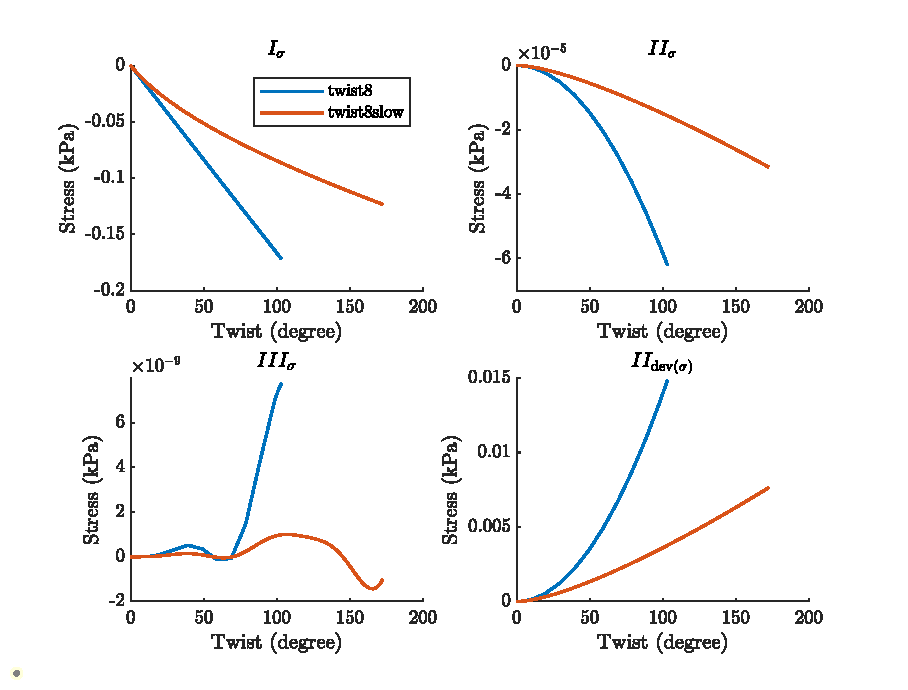
\includegraphics[width = 0.95\textwidth]{2EL_column_twist8.eps}} \label{fig:twist8} 
    \subfloat[]{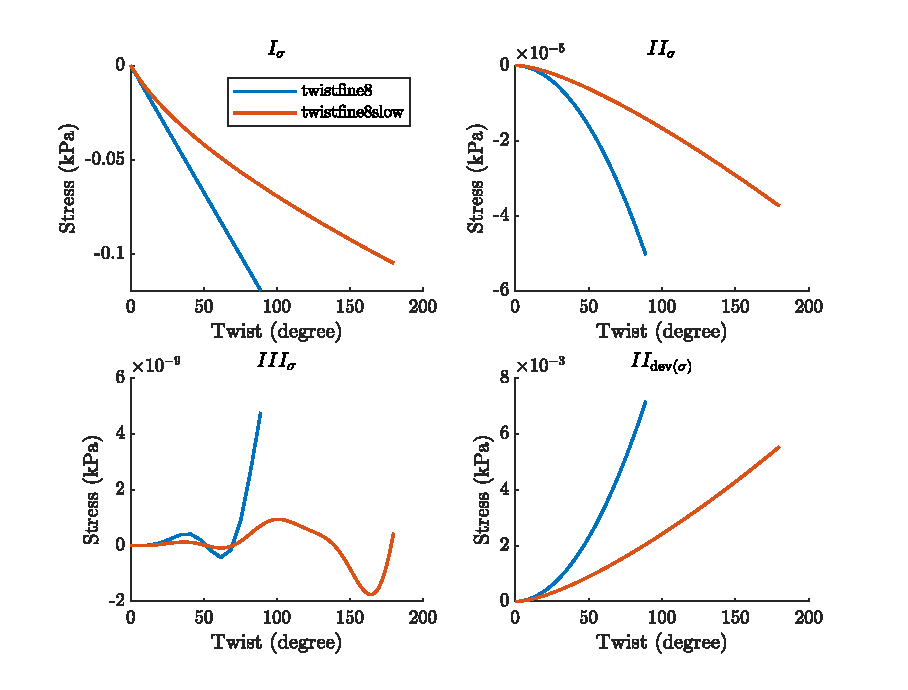
\includegraphics[width = 0.95\textwidth]{2EL_column_twistfine8.eps}} \label{fig:twistfine8}
\end{figure}
\begin{figure}[htpb]\ContinuedFloat
    \centering
    \subfloat[]{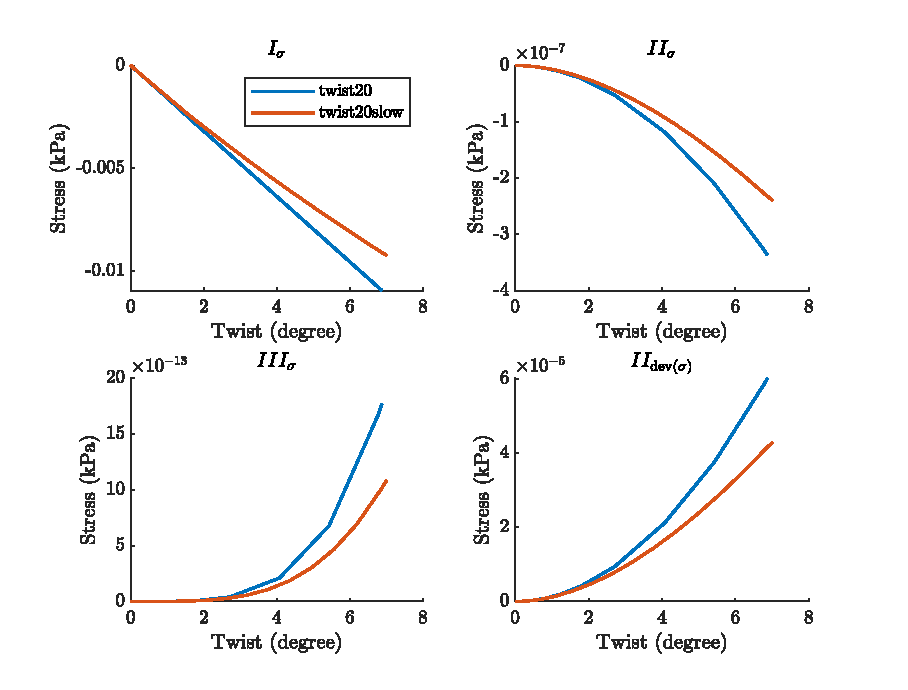
\includegraphics[width = 0.95\textwidth]{2EL_column_twist20.eps}} \label{fig:twist20}
    \caption[Column twisting simulation results]{Column twisting simulation results in ABAQUS discretized with (a) 576 C3D8H, (b) 9000 C3D8H and (c) 576 C3D20H elements using viscoelastic material model with two relaxation mechanisms \((k=2)\) and material parameters \(\bm{x}_{p}\) for \(2\mathrm{EL}_{\mathrm{NR}}\) (\cref{tab:opt_param_sets})}\label{fig:column_twisting}
\end{figure}




